% В этом документе преамбула

%%% Работа с русским языком
\usepackage{cmap}					% поиск в PDF
\usepackage{mathtext} 				% русские буквы в формулах
\usepackage[T2A]{fontenc}			% кодировка
\usepackage[utf8]{inputenc}			% кодировка исходного текста
\usepackage[english,russian]{babel}	% локализация и переносы
\usepackage{indentfirst}			% чтобы первый абзац в разделе отбивался красной строкой
\frenchspacing						% тонкая настройка пробелов

%%% Приведение начертания букв и знаков к русской типографской традиции
\renewcommand{\epsilon}{\ensuremath{\varepsilon}}
\renewcommand{\phi}{\ensuremath{\varphi}}			% буквы "эпсилон"
\renewcommand{\kappa}{\ensuremath{\varkappa}}		% буквы "каппа"
\renewcommand{\le}{\ensuremath{\leqslant}}			% знак меньше или равно
\renewcommand{\leq}{\ensuremath{\leqslant}}			% знак меньше или равно
\renewcommand{\ge}{\ensuremath{\geqslant}}			% знак больше или равно
\renewcommand{\geq}{\ensuremath{\geqslant}}			% знак больше или равно
\renewcommand{\emptyset}{\varnothing}				% знак пустого множества

%%% Дополнительная работа с математикой
\usepackage{amsmath,amsfonts,amssymb,amsthm,mathtools} % AMS
\usepackage{icomma} % "Умная" запятая: $0,2$ --- число, $0, 2$ --- перечисление

%% Номера формул
\mathtoolsset{showonlyrefs=true} % Показывать номера только у тех формул, на которые есть \eqref{} в тексте.

%% Свои команды

% операции, не определённые (или имеющие иные обохначения) в мат. пакетах
\DeclareMathOperator{\sgn}{\mathop{sgn}}				% ф-ия sgn
\renewcommand{\tg}{\mathop{\mathrm{tg}}\nolimits}		% обозначение тангенса

%% Перенос знаков в формулах (по Львовскому)
\newcommand*{\hm}[1]{#1\nobreak\discretionary{}
{\hbox{$\mathsurround=0pt #1$}}{}}

%%% Работа с картинками
\usepackage{graphicx}  % Для вставки рисунков
\graphicspath{{images/}{images2/}}  % папки с картинками
\setlength\fboxsep{3pt} % Отступ рамки \fbox{} от рисунка
\setlength\fboxrule{1pt} % Толщина линий рамки \fbox{}
\usepackage{wrapfig} % Обтекание рисунков текстом

%%% Работа с таблицами
\usepackage{array,tabularx,tabulary,booktabs} % Дополнительная работа с таблицами
\usepackage{longtable}  % Длинные таблицы
\usepackage{multirow} % Слияние строк в таблице

%%% Теоремы
\theoremstyle{plain} % Это стиль по умолчанию, его можно не переопределять.
\newtheorem{theorem}{Теорема}[section]
\newtheorem{lemma}{Лемма}[section]
\newtheorem{definition}[theorem]{Определение}
\newtheorem{property}{Свойство}
 
\theoremstyle{definition} % "Определение"
\newtheorem{corollary}{Следствие}[theorem]
\newtheorem{exmp}{Пример}[section]
 
\theoremstyle{remark} % "Примечание"
\newtheorem*{nonum}{Решение}
\newtheorem*{evidence}{Доказательство}
\newtheorem*{remark}{Примечание}

%%% Программирование
\usepackage{etoolbox} % логические операторы

%%% Страница
\usepackage{extsizes} % Возможность сделать 14-й шрифт
\usepackage{geometry} % Простой способ задавать поля
	\geometry{top=25mm}
	\geometry{bottom=35mm}
	\geometry{left=35mm}
	\geometry{right=20mm}

%\usepackage{fancyhdr} % Колонтитулы
% 	\pagestyle{fancy}
 	%\renewcommand{\headrulewidth}{0pt}  % Толщина линейки, отчеркивающей верхний колонтитул
% 	\lfoot{Нижний левый}
% 	\rfoot{Нижний правый}
% 	\rhead{Верхний правый}
% 	\chead{Верхний в центре}
% 	\lhead{Верхний левый}
%	\cfoot{Нижний в центре} % По умолчанию здесь номер страницы

\usepackage{setspace} % Интерлиньяж (межстрочные интервалы)
%\onehalfspacing % Интерлиньяж 1.5
%\doublespacing % Интерлиньяж 2
%\singlespacing % Интерлиньяж 1

\usepackage{lastpage} % Узнать, сколько всего страниц в документе.

\usepackage{soulutf8} % Модификаторы начертания

\usepackage{hyperref}
\usepackage[usenames,dvipsnames,svgnames,table,rgb]{xcolor}
\hypersetup{				% Гиперссылки
    unicode=true,           % русские буквы в раздела PDF
    pdftitle={Заголовок},   % Заголовок
    pdfauthor={Автор},      % Автор
    pdfsubject={Тема},      % Тема
    pdfcreator={Создатель}, % Создатель
    pdfproducer={Производитель}, % Производитель
    pdfkeywords={keyword1} {key2} {key3}, % Ключевые слова
    colorlinks=true,       	% false: ссылки в рамках; true: цветные ссылки
    linkcolor=MidnightBlue,          % внутренние ссылки
    citecolor=black,        % на библиографию
    filecolor=magenta,      % на файлы
    urlcolor=blue           % на URL
}

\usepackage{csquotes} % Еще инструменты для ссылок

%\usepackage[style=authoryear,maxcitenames=2,backend=biber,sorting=nty]{biblatex}

\usepackage{multicol} % Несколько колонок

%%% Работа с графикой
\usepackage{tikz}
\usetikzlibrary{calc}
\usepackage{tkz-euclide}
\usetikzlibrary{arrows}
\usepackage{pgfplots}
\usepackage{pgfplotstable}

%%% Настройка подписей к плавающим объектам
\usepackage{floatrow}	% размещение
\usepackage{caption}	% начертание
\captionsetup[figure]{labelfont=bf,textfont=it,font=footnotesize}	% нумерация и надпись курсивом
% для подфигур: заголовок подписи полужирный, текст заголовка обычный
% выравнивание является неровным (т.е. выровненным по левому краю)
% singlelinecheck = off означает, что настройка выравнивания используется, даже если заголовок имеет длину только одну строку.
% если singlelinecheck = on, то заголовок всегда центрируется, когда заголовок состоит только из одной строки.
\captionsetup[subfigure]{labelfont=bf,textfont=normalfont,singlelinecheck=off,justification=raggedright}

%%% Stuff для графиков и рисунков



\title{Теория вероятностей и мат. статистика \\ ИДЗ4}
\date{23.05.2020}
\author{Почаев Никита Алексеевич, гр. 8381 \\ \href{mailto:pochaev.nik@gmail.com}{pochaev.nik@gmail.com} \\ Преподаватель: Малов Сергей Васильевич}

\begin{document}
	
\renewcommand{\figurename}{Рисунок}

\maketitle

\begin{figure}[H]
	\center{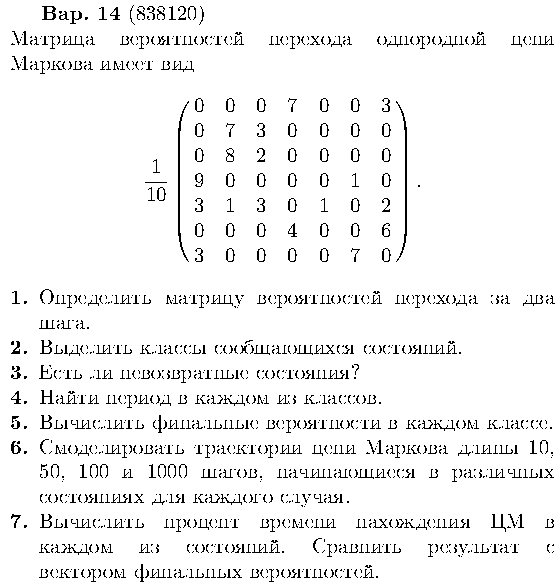
\includegraphics[scale=1]{./media/Задание.pdf}}
\end{figure}
\newpage
Для удобства построим граф данной цепи.
\begin{figure}[H]
	\center{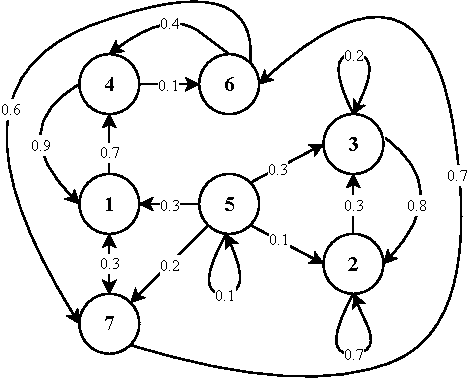
\includegraphics[scale=1.3]{./media/scheme.pdf}}
\end{figure}

\subsection*{Задача 1.}

\[
\mathbb{P}^{(2)} = \mathbb{P}^2 =
\frac{1}{100}
\begin{bmatrix}
	72 & 0  & 0  & 0  & 0 & 28 & 0  \\
	0  & 73 & 27 & 0  & 0 & 0  & 0  \\
	0  & 72 & 28 & 0  & 0 & 0  & 0  \\
	0  & 0  & 0  & 67 & 0 & 0  & 33 \\
	9  & 32 & 12 & 21 & 1 & 14 & 11 \\
	54 & 0  & 0  & 0  & 0 & 46 & 0  \\
	0  & 0  & 0  & 49 & 0 & 0  & 51
\end{bmatrix}
\]

Проверим: сумма элементом каждой строки равна 1.

\subsection*{Задача 2.}

Данная марковская цепь состоит класса сообщающихся состояний: $\{ v_1, v_4, v_6, v_7 \}$
\begin{table}[H]
	\centering
	\begin{tabular}{|c|c|}
		\hline
		\textbf{Состояние} & \textbf{Док-во}                            \\ \hline
		$v_1 \eq v_4$      & $v_1 \to v_4, v_4 \to v_1$                 \\ \hline
		$v_1 \eq v_7$      & $v_1 \to v_7, v_7 \to v_1$                 \\ \hline
		$v_4 \eq v_6$      & $v_4 \to v_6, v_6 \to v_4$                 \\ \hline
		$v_6 \eq v_7$      & $v_6 \to v_7, v_7 \to v_2 \to v_4 \to v_6$ \\ \hline
		$v_1 \eq v_6$      & $v_1 \to v_4 \to v_6, v_6 \to v_4 \to v_1$ \\ \hline
		$v_4 \eq v_7$      & $v_4 \to v_1 \to v_7, v_7 \to v_1 \to v_4$ \\ \hline
	\end{tabular}
\end{table}
а также из другого класса $\{ v_2, v_3 \}: v_2 \to v_3, v_3 \to v_2$ (данные классы не пересекаются: ни одна вершина одного классе не достижима из вершины другого класса). Вершина $v_5$ является недостижимой из любой вершины ($\exists$ пути из неё, но не в неё) и $\Rightarrow$ несущественной.

\subsection*{Задача 3.}

Т.к. несущественные состояния невозвратны, то $v_5$ - невозвратная.

\subsection*{Задача 4.}

Т.к. в классе $\{ v_2, v_3 \}$ есть петля, его период будет равен 1, период же другого класса равен 2, т.к. НОД периодов всех состояний равен 2-м.

\subsection*{Задача 5.}

\subsubsection*{Класс 1.}

\noindent Класс: $\{ v_1, v_4, v_6, v_7 \}$. Вектор финальных состояний вероятностей: $x = [p_1, p_4, p_6, p_7]$.

\[
\mathbb{P}'_{ \{ v_1, v_4, v_6, v_7 \} } = \mathbb{P} = \frac{1}{10}
\begin{bmatrix}
0 & 7 & 0 & 3 \\
9 & 0 & 1 & 0 \\
0 & 4 & 0 & 6 \\
3 & 0 & 7 & 0
\end{bmatrix}
\]

В периодической цепи финальные вероятности не существуют, следовательно, возведём матрицу в квадрат и таким образом получим ЦМ за два шага.

\[
\mathbb{P}^2 = \frac{1}{100}
\begin{bmatrix}
72 & 0  & 28 & 0  \\
0  & 67 & 0  & 33 \\
54 & 0  & 46 & 0  \\
0  & 49 & 0  & 51
\end{bmatrix}
\]

Для удобства определения подклассов рассмотрим графическое представление.
\begin{figure}[H]
	\center{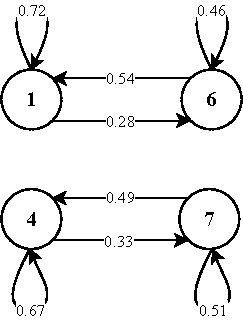
\includegraphics[scale=1]{./media/scheme_2.pdf}}
\end{figure}

Вычислим финальные состояния в каждом классе.
\begin{enumerate}
	\item Класс $\{ 1,6 \}$
	\[ P_{\{1,6\}} = \frac{1}{100}
	\begin{bmatrix}
	72 & 28 \\
	54 & 46
	\end{bmatrix}
	\]
	\[
	\begin{cases}
	100 p_1 = 72 p_1 + 54 p_6 \\
	100 p_6 = 28 p_1 + 46 p_6 \\
	p_1 + p_6 = 1
	\end{cases}
	\Rightarrow
	\begin{cases}
	p_1 = \frac{27}{41} \\
	p_6 = \frac{14}{41}
	\end{cases}
	\]
	\item Класс $\{ 4,7 \}$
	\[ P_{\{4,7\}} = \frac{1}{100}
	\begin{bmatrix}
	67 & 33 \\
	49 & 51
	\end{bmatrix}
	\]
	\[
	\begin{cases}
	100 p_4 = 67 p_4 + 49 p_7 \\
	100 p_7 = 33 p_4 + 51 p_7 \\
	p_4 + p_7 = 1
	\end{cases}
	\Rightarrow
	\begin{cases}
	p_4 = \frac{49}{82} \\
	p_7 = \frac{33}{82}
	\end{cases}
	\]
\end{enumerate}

\subsubsection*{Класс 2.}

\noindent Класс: $\{ v_2, v_3 \}$. Вектор финальных состояний вероятностей: $x = [p_2, p_3]$.

\[
\mathbb{P}_{ \{ v_2, v_3 \} } = \frac{1}{10}
\begin{bmatrix}
7 & 3 \\
8 & 2
\end{bmatrix}
\]

\[
\begin{bmatrix}
7 & 8 \\
3 & 2
\end{bmatrix}
\begin{bmatrix}
p_2 \\ p_3
\end{bmatrix}
=
\begin{bmatrix}
10 p_2 \\ 10 p_3
\end{bmatrix}
~~~~~~~~~
\begin{bmatrix}
-3 & 8 \\
3 & -8
\end{bmatrix}
\begin{bmatrix}
p_2 \\ p_3
\end{bmatrix}
=
\begin{bmatrix}
0 \\ 0
\end{bmatrix}
\]
\[ p_2 + p_3 = 1 \]
\[
\left[
\begin{array}{rr|r}
-3 & 8 & 0 \\
3 & -8 & 0 \\
1 & 1 & 1
\end{array}
\right]
\]
В результате:
\[ p_2 = \frac{8}{11}, p_3 = \frac{3}{11} \]

\end{document} 